\chapter{The simplex method}
\label{cha:simplex-method}


In this chapter we describe the simplex method. The task is to solve a linear program 
\begin{equation}
  \label{eq:s-1}
  \max\{c^Tx \colon x \in \R^n, \,  Ax \leq b\}.
\end{equation}
We make the following assumption.
\begin{quote}
  The matrix $A \in\R^{m\times n}$ is of full column-rank. In other words, the columns of $A$ are linearly independent. 
\end{quote}
%
This assumption is not a restriction, since we can solve  the following equivalent linear program instead, where each $x_i$ is represented as the difference of two positive values $x_i = x_i^+ - x_i^-$. 
\begin{equation}
  \label{eq:s-2}
    \max\{c^Tx^+-c^Tx^- \colon x^+ ,x^- \in \R^n, \,  Ax^+-Ax^- \leq b, x^+ \geq 0, \, x^- \geq 0\}.
\end{equation}
The constraint matrix of the linear program~\eqref{eq:s-2} in inequality standard form is 
\begin{displaymath}
  \begin{pmatrix}
    A & -A \\
    -I_n & \mathbf{0} \\
    \mathbf{0} & -I_n
  \end{pmatrix},
\end{displaymath}
where $I_n$ is the $n\times n$ identity matrix and $\mathbf{0}$ is the $n\times n$ all-zero matrix. Clearly this matrix has linearly independent columns. 


\section{Adjacent vertices}
\label{sec:adjacent-vertices}


Let $P = \{x \in \R^n \colon Ax \leq b\}$ be the polyhedron of feasible solutions of \eqref{eq:s-1}. 

\begin{definition}
  \label{def:s-1}
  Two extreme points $x_1\neq x_2$ of $P$ are \emph{adjacent}, if there exists a valid inequality $d^Tx \leq \delta$ of $P$ such that 
  \begin{displaymath}
    P \cap \{x \in \R^n \colon d^Tx = \delta\} = \{ \lambda x_1 + (1-\lambda)x_2 \colon \lambda \in [0,1]\}. 
  \end{displaymath}
\end{definition}
In other words, $x_1 \neq x_2$ are adjacent if there exists a valid inequality for $P$ such that the points of $P$ that satisfy this inequality with equality are exactly the line-segment spanned by $x_1$ and $x_2$. 

Similar to the characterization of extreme points in Theorem~\ref{thr:1}, we can state and prove the following theorem. 

\begin{theorem}
  \label{thr:s-3}
  Two distinct vertices $x_1$ and $x_2$ of $P$ are adjacent if and
  only if there exists a sub-system $A'x \leq b'$ of $Ax \leq b$ such
  that
  \begin{enumerate}[i)]
  \item $A' \in \R^{(n-1)\times n}$ and the rows of $A'$ are linearly
    independent. \label{item:s-4}
  \item $x_1$ and $x_2$ satisfy $A'x \leq b'$ with
    equality. \label{item:s-3}
  \end{enumerate}
\end{theorem}

\begin{proof}
  Suppose that $x_1 \neq x_2$ are adjacent and suppose that $d^Tx \leq
  \delta$ is a valid inequality that asserts this fact. Consider the sub-system $\wt{A} x \leq \wt{b}$ of inequalities  of $Ax \leq b$ that are satisfied by $1/2 (x_1 + x_2)$ with equality. These are the inequalities that are satisfied by all points on the line-segment with equality. Since  $\wt{A}(x_1-x_2) = 0$, one has $\rank(\wt{A}) \leq n-1$. If $\rank(\wt{A}) < n-1$, then there exists a $v \in \R^n$ that is linearly independent from $(x_1-x_2)$ that satisfies $\wt{A} v = 0$. Consequently there exist a $\varepsilon >0$ such that 
  \begin{equation}
    \label{s:3}    
    \{ \frac{1}{2}(x_1+x_2) + \mu_1 (x_1-x_2) + \mu_2 v \colon -\varepsilon \leq \mu_1,\mu_2 \leq \varepsilon \} \subseteq P. 
  \end{equation}
All points of the set~\eqref{s:3} satisfy $d^Tx \leq \delta$ with equality and they are not a subset of the line-segment spanned by $x_1$ and $x_2$. From this we conclude that $\rank(\wt{A}) = n-1$ which implies that there exists a sub-system $A'x \leq b'$ satisfying~\ref{item:s-4}) and \ref{item:s-3}). 

Suppose on the other hand that there exists a sub-system $A'x \leq b'$
that satisfies \ref{item:s-4}) and \ref{item:s-3}).  The line spanned
by $x_1$ and $x_2$ is the set of points of $\R^n$ that satisfies $A'x
= b'$ and the intersection of this line with $P$ is, since $x_1$
and $x_2$ are vertices, the line-segment spanned by these two points.

The inequality $\mathbf{1}^T A'x \leq \mathbf{1}^T b'$ is valid for $P$ and is satisfied by the line-segment spanned by $x_1$ and $x_2$ with equality. Let $y^* \in P$ be a point  that does not lie on the line segment. Then one of the inequalities of $A'x \leq b'$ is satisfied by $y^*$ with strict inequality and thus $y^*$ does not satisfy $d^Tx \leq \delta$ with equality. 
\end{proof}




\section{Bases, feasible bases and vertices}
\label{sec:non-degenerate-case}

We will frequently use the following notation. Let $B \subseteq \{1,\dots,m\}$ then $A_B \in \R^{|B| \times n}$ is the matrix consisting of the rows of $A$ that are indexed by   $B$ and $b_B \in \R^{|B|}$  is the vector whose components are the ones of $b$ indexed by $B$.


\begin{example}
  \label{ex;pyth-1}
For 
$    A = 
    \begin{pmatrix}
      3 & 2  \\
      7 & 1\\
      8 & 4\\
    \end{pmatrix}$,  $b = 
    \begin{pmatrix}
      3 \\ 2\\ 6
    \end{pmatrix}$ 
    and  $B = \{2,3\}$, one has
    \begin{displaymath}
    A_B =  \begin{pmatrix}
          7 & 1\\
      8 & 4\\
    \end{pmatrix} \text{ and }  b_B = 
    \begin{pmatrix}
      2\\ 6
    \end{pmatrix}.          
    \end{displaymath}

\medskip
\noindent     
A \emph{python implementation} based on the {\tt sympy} package of the above is as follows. Notice that the index set represented by a list {\tt B} here is starting at $1$, since the first row of a matrix in {\tt sympy} is indexed by $0$.  
\begin{lstlisting}[language=python]
from sympy import *
A = Matrix([[3,2],[7,1],[8,4]])
b =  Matrix([3,2,6])

B = [1,2]

pprint(A[B,:])
pprint(b[B,:]) 
\end{lstlisting}
\end{example}


    \begin{definition}
      \label{def:s1-1}
      An index set $B \subseteq \{1,\dots,m\}$ is a \emph{basis} if
      $|B| = n$ and $A_B$ is non-singular. If in addition $x^* =
      A_B^{-1} b_B$ is feasible, then $B$ is called a \emph{feasible
        basis}.
    \end{definition}

    Theorem~\ref{thr:1} implies that every vertex $x^*$ of $P = \{x
    \in \R^n \colon Ax \leq b\}$ is \emph{represented} by a basis $B$,
    i.e. $x^*$ is the unique solution of $A_Bx^* = b_B$. This
    representation however must not be unique, see
    Figure~\ref{fig:7}. We say that a linear program is \emph{degenerate}, if
    there exists a basic solution $x^* \in \R^n$ that satisfies $n+1$
    inequalities with equality. Otherwise the linear program is called
    \emph{non-degenerate}. If the linear program is non-degenerate,
    then each vertex is represented by \emph{exactly one} basis.

    \begin{figure}
      \centering
      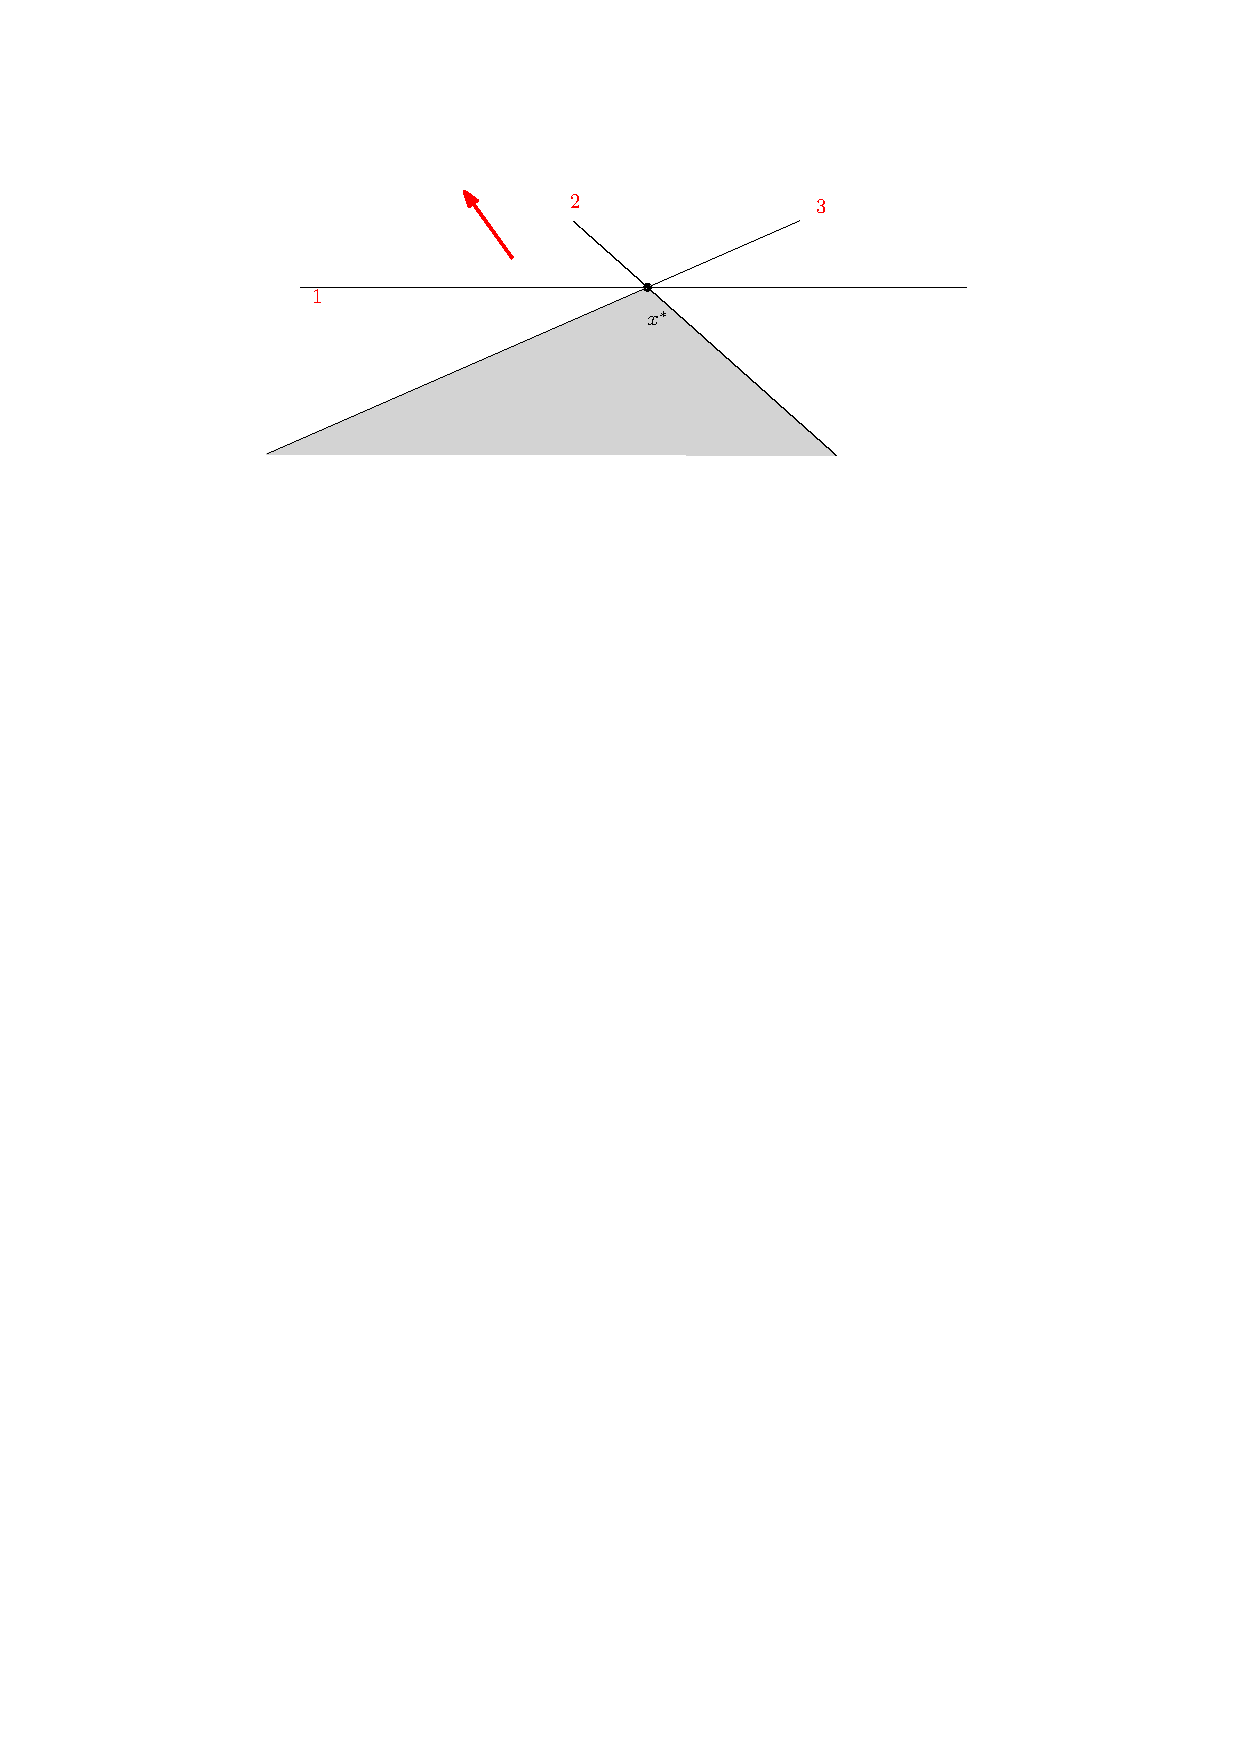
\includegraphics[height=3cm]{figures/Degenerate.pdf}
      \caption{The vertex $x^*$ is represented by each choice of two of the three tight constraints. The linear program is degenerate. The red vector is the objective function vector and the red labels are the indices of the constraints.}
      \label{fig:7}
    \end{figure}



    \begin{definition}
      \label{def:s-2}
       A basis $B$ is called \emph{optimal} if it is feasible and the
       unique $\lambda \in \setR^m$ 
       with 
       \begin{equation}
         \label{eq:s-5}
         \lambda^T A =  c^T \, \, \text{ and } \lambda_i = 0, \, i \notin B 
       \end{equation}
       satisfies $\lambda\geq0$. 
     \end{definition}


The basis $\{1,2\}$ in Figure~\ref{fig:7} is not optimal whereas the bases $\{2,3\}$ and $\{1,3\}$ are optimal bases. 


\begin{theorem}
  \label{thr:s-4}
  If $B$ is an optimal basis, then $x^* = A_B^{-1} b_B$ is an optimal solution of the linear program~\eqref{eq:s-1}. 
\end{theorem}

\begin{proof}
  The inequality $\lambda^T A x \leq \lambda^T b$ is valid for $P = \{x \in \R^n \colon Ax \leq b\}$. But $\lambda^T A =c^T$ and $\lambda^T b = \lambda^T Ax^* = c^Tx^*$. Consequently $x^*$ is an optimal solution of the linear program \eqref{eq:s-1}. 
\end{proof}


\section{Moving to an improving vertex}
\label{sec:moving-an-improving}

Suppose now that $B$ is a feasible but not optimal basis. Then the
unique $\lambda$ satisfying~\eqref{eq:s-5} has a negative component
$\lambda_i<0$ for some $i \in B$. The idea is now to move from $x^*_B
= A_B^{-1}b_B$ by remaining tight at all constraints indexed by $B$
except for $i$.

There is only one way this can be achieved. Namely by moving in the unique direction $d$ with
\begin{displaymath}
  a_j^T d =
  \begin{cases}
    0 & \text{ for } j \in B \setminus \{i\} \\
    -1 & \text{ if } j =i.
  \end{cases}
\end{displaymath}

When we do this, we follow the ray $x^*_B + \varepsilon \cdot d$ with $\varepsilon
\geq 0$. What happens to the objective function, as $\varepsilon$ grows? Since
$c^Td = \lambda^TA d = -\lambda_i >0$, the objective function strictly
grows with growing $\varepsilon$. There are now two cases. 

At some point, we hit the boundary of a constraint and further increase of $\varepsilon$ results in an infeasible point. Let $K \subseteq \{ 1,\dots,m\}$ be the set of indices 
\begin{equation}
  \label{eq:s-6}
  K = \{ k \colon 1 \leq k \leq m, \,a_k^T d >0\}. 
\end{equation}
Those are the indices of constraints that, at some point, will be violated. We can increase $\varepsilon$ until 
\begin{equation}
  \label{eq:s-8}
  \varepsilon^* = \min_{k \in K} \{ (b_k - a_k^Tx^*) / a_k^Td\}. 
\end{equation}
Now pick any $k \in K$ for which this minimum is achieved and set $B' = B \setminus \{i\} \cup \{k\}$. This is a feasible basis, $d$ is orthogonal to all rows  indexed by $B \setminus \{i\}$ but not to $a_k$. 

In the case where there is no constraint that puts an upper bound on $\varepsilon$, then the linear program is \emph{unbounded}. 
We have described one iteration of the simplex algorithm. We iterate this procedure until an optimal solution is found. 



\begin{example}
  \label{example:moving}
  Consider the linear program $\max\{ c^Tx : A≤b, \,x∈ℝ^3 \}$ with
  
  \begin{displaymath}
    A  =\begin{pmatrix}1 & 2 & 2\\2 & 1 & 2\\2 & 2 & 1\\-1 & 0 & 0\\0 & -1 & 0\\0 & 0 & -1\end{pmatrix}, \, b = 
    \begin{pmatrix}10\\14\\11\\0\\0\\0\end{pmatrix} \text{ and } c =
    \begin{pmatrix}
      6\\14\\13
    \end{pmatrix}
  \end{displaymath}
  with starting basis
  \begin{displaymath}
    B = \{1,2,3\}. 
  \end{displaymath}
  One has
  \begin{displaymath}
    A_B = \begin{pmatrix}1 & 2 & 2\\2 & 1 & 2\\2 & 2 & 1\end{pmatrix} b_B = \begin{pmatrix}10\\14\\11\end{pmatrix} \text{ and } x^*_B = \begin{pmatrix}4\\0\\3\end{pmatrix}. 
  \end{displaymath}
  For $λ_B$ one obtains
  \begin{displaymath}
    λ_B = \begin{pmatrix}\frac{36}{5}\\- \frac{4}{5}\\\frac{1}{5}\end{pmatrix}. 
  \end{displaymath}
  From this it follows that $2$ leaves the basis. The direction $d$ is the solution of the system
  \begin{displaymath}
     A_B d =
     \begin{pmatrix}
       0\\-1\\0
     \end{pmatrix}. 
   \end{displaymath}
   One has
   \begin{displaymath}
     d = \begin{pmatrix}- \frac{2}{5}\\\frac{3}{5}\\- \frac{2}{5}\end{pmatrix}. 
   \end{displaymath}
  


The vector $Ad$ is 
\begin{displaymath}
  A ⋅ d = \begin{pmatrix}0\\-1\\0\\\frac{2}{5}\\- \frac{3}{5}\\\frac{2}{5}\end{pmatrix}. 
\end{displaymath}
and one has
\begin{displaymath}
  b-Ax^* = 
\begin{pmatrix}0\\0\\0\\4\\0\\3\end{pmatrix}.
\end{displaymath}
This means that $6$ enters the basis. 

\end{example}



\begin{figure}
  \centering
\begin{lstlisting}[language=python]
from sympy import *

A = Matrix([[1, 2, 2],
             [2, 1, 2],
             [2, 2, 1],            
             [-1, 0, 0],
             [0, -1, 0],
             [0, 0, -1]])
 
b = Matrix([10,14,11,0,0,0])
c = Matrix([6,14,13])
r = Matrix([0,-1,0])

B = [0,1,2]
 
A_B = A[B,:] 
b_B = b[B,:]
 
x =  A_B.solve(b_B) 
l = A_B.transpose().solve(c)
d = A_B.transpose().solve(r)

L = {"A_B =":A_B, "b_B =":b_B, "x^*=":x, "\lambda_B =":l , "d = ":d}

for key, value in L.items():
    print (key) 
    pprint(value) 
\end{lstlisting}

  \caption{A partial python code for example~\ref{example:moving}.}
\end{figure}\label{fig:code-2}

\newpage
\begin{algorithm}[Simplex algorithm]
  \begin{tabbing}
    Start with feasible basis $B$ \\[1ex]
    {\tt while} \= $B$ is not optimal \\ [.7ex]
    \> Let $i \in B$ be index with $\lambda_i<0$ \\
    \> Compute  $d \in \setR^n$ with $a_j^T d = 0, \, j \in B \setminus\{i\}$
    and $a_i^T d = -1$ \\ 
    \> Determine $K = \{ k \colon 1 \leq k \leq m, \, a_k^Td >0\}$\\[.7ex]  
    \> {\tt if} \= $K = \emptyset$ \\   
    \> \> \emph{assert LP unbounded} \\
    \> {\tt else} \\
    \> \> Let $k \in K$ index where 
    $
    \displaystyle \min_{k \in K} (b_k - a_k^Tx^*)/a_k^Td
    $
    is attained \\ %(with  $x^* = A_B^{-1}b_B$)
    
    \> \>\emph{update} $B := B \setminus\{i\} \cup \{k\}$             
  \end{tabbing}
  
\end{algorithm}
  


\begin{theorem}
  \label{thr:s-5}
  If the linear program~\eqref{eq:s-1} is non-degenerate, then the
  simplex algorithm terminates.
\end{theorem}

\begin{proof}
  In the non-degenerate case, $\varepsilon^*>0$ and the simplex
  algorithm makes progress, i.e., the objective function value
  strictly increases after each iteration. Since there is only a
  finite number of vertices, the algorithm terminates.
\end{proof}

  
\section{Termination in the degenerate case}
\label{sec:term-degen-case}


In the case where the linear program~\eqref{eq:s-1} is degenerate, we cannot argue that the objective function value increases each iteration and that the simplex algorithm terminates. However, the simplex algorithm leaves us some choice. Namely, there can be several indices $i \in B$ such that $\lambda_i<0$. Also, there could be several indices $k \in K$ attaining the minimum in \eqref{eq:s-8}. If one adheres to the  \emph{smallest index rule}, then one can prove termination of the simplex algorithm also in the degenerate case. One iteration of the simplex algorithm is now as follows. 



\begin{algorithm}[Simplex algorithm with the smallest index rule]
 \begin{tabbing}
      Start with feasible basis $B$ \\[1ex]
      {\tt while} \= $B$ is not optimal \\ [.7ex]
      \> Compute $\lambda \in \setR^n$ such that $\lambda^TA_B = c^T$ \\
      \> Let $i^* \in B$ be the \emph{ smallest index} with $\lambda_i<0$ \\
      \> Compute  $d \in \setR^n$ with $a_j^T d = 0, \, j \in B \setminus\{i^*\}$
      and $a_{i^*}^T d = -1$ \\ 
      \> Determine $K = \{ k \colon 1 \leq k \leq m, \, a_k^Td >0\}$\\[.7ex]  
      \> {\tt if} \= $K = \emptyset$ \\   
      \> \> \emph{assert LP unbounded} \\
      \> {\tt else} \\
      \> \> Let $k^* \in K$ the \emph{smallest index} where 
     $
        \displaystyle \min_{k \in K} (b_k - a_k^Tx^*)/a_k^Td
      $
      is attained \\ %(with  $x^* = A_B^{-1}b_B$)

      \> \>\emph{update} $B := B \setminus\{i^*\} \cup \{k^*\}$             
    \end{tabbing}
    
  \end{algorithm}
  



  \begin{theorem}
    \label{thr:3}
    The simplex algorithm with the smallest index rule terminates. 
  \end{theorem}

  \begin{proof}
    We suppose that the simplex algorithm does not terminate. This means that the simplex algorithm iterates through a sequence of bases 
    \begin{displaymath}
      B_0,B_1,\dots,B_k
    \end{displaymath}
    with $B_k = B_0$. Inspecting two succeeding bases $B_\ell$ and
    $B_{\ell+1}$ for $0\leq \ell \leq k-1$, one has $B_{\ell+1}
    =B_{\ell} \setminus \{i\} \cup \{j\}$, i.e., $i$ \emph{leaves}
    and $j$ \emph{enters} $B_{\ell}$. Now let $j$ be \emph{the largest
      index} that leaves on that sequence. Since $B_0 = B_k$, $j$ also
    enters again at some point. Let $p$ and $q$ be the indices of
    bases, $0 \leq p,q <k$ where $j$ leaves and enters respectively. 

    Let $\lambda^{(p)}$ and $d^{(q)}$ be the corresponding $\lambda$ and $d$
    vectors from the iteration $p$ and $q$ of the simplex algorithm
    respectively. Since ${\lambda^{(p)}}^T A = c^T$ and $c^T d^{(q)}>0$ we conclude 
    \begin{equation}
      \label{eq:s15-1}
      {\lambda^{(p)}}^T A d^{(q)} >0.
    \end{equation}
    Let $i \in B_p$ be an index with 
    \begin{equation}
      \label{eq:s-15-2}
      \lambda^{(p)}_i a_i d^{(q)} >0
    \end{equation}
    where $a_i$ denotes the $i$-th row of $A$. 


    We now distinguish three cases. Let us suppose that $i>j$. Then,
    since $j$ is the largest index that ever leaves or enters one has
    that $i$ is also an element of $B_q$ implying that $ a_i d^{(q)}$
    is $0$ or $-1$. It cannot be $-1$, since this would mean that $i$
    leaves $B_q$ contradictory to the choice of $j$.

    Suppose then that $i<j$. Then $\lambda_i^{(p)}>0$ since $j$ is the
    smallest index that can leave the basis $B_p$. But $a_id^{(q)} >0$
    is not possible, otherwise index $i$ is an index where the minimum
    ($\varepsilon^* = 0$) in \eqref{eq:s-8} is attained and $j>i$ is
    the smallest index where this minimum is attained. Thus this case
    can also be ruled out.

    Finally, if $i=j$, then $\lambda_i^{(p)} <0$ and $a_i d^{(q)}>0$
    which also contradicts~\eqref{eq:s-15-2}.
  \end{proof}


\section{Finding an initial basic feasible solution}
\label{sec:finding-an-initial}

The simplex algorithm starts with a feasible basis. How can such a feasible basis be determined? In fact, this can be done with an auxiliary linear program. 

Any linear program has an equivalent form 
\begin{equation}
  \label{eq:s-3}
  \max\{ c^Tx \colon Ax \leq b, \, x \geq 0\}. 
\end{equation}
  We want to find an initial feasible basis for this linear program. Suppose first that we re-write the constraints $Ax \leq b$ as $A_1x\leq b_1$ and $A_2x\leq b_2$ with $b_1 \geq 0$ and $b_2<0$. Now consider the following linear program
  \begin{equation}
    \label{eq:s-151}    
  \min\{ \mathbf{1}^Ty \colon A_1x \leq b_1, \, A_2x \leq b_2 +y, \, x,y \geq 0, y \leq -b_2\}. 
\end{equation}
An initial basic feasible solution is $x=0$ and $y= -b_2$ with the basis corresponding to the inequalities $x\geq 0$ and $y \leq -b_2$. The simplex algorithm applied to this linear program terminates. It finds an optimal solution with objective value $0$ if and only if the original linear program is feasible. Let $B$ be the optimal basis in this case. Then $B$ without the indices corresponding to the constraints $y\geq 0$ is a feasible basis for the linear program~\eqref{eq:s-3}.  This follows from the fact that the rows of $A$ indexed by $B$ must be linearly independent. If the corresponding rank was smaller than $n$, then the rank of the rows of the auxiliary linear program~\eqref{eq:s-151} indexed by $B$ would be smaller than $n+k$, where $k$ is the number of rows of $A_2$. 


\section{Removing degeneracy by perturbation}
\label{sec:remov-degen-pert}

In the following, we derive an alternative pivoting rule that also ensures termination of the simplex algorithm. We begin by \emph{perturbing} the right-hand-sides of our constraints 
\begin{equation}
  \label{eq:pert-2}
  Ax \leq b
\end{equation}
by adding a vector $p_\eps$ 
\begin{equation}
  \label{eq:per-1}
  Ax \leq b + p_\eps 
\end{equation}
where $p_\eps$ is the vector 
\begin{displaymath}
p_\eps = 
  \begin{pmatrix}
    \eps\\ \eps^2\\ \vdots \\ \eps^m
  \end{pmatrix}.
\end{displaymath}

\begin{lemma}
  \label{lem:per-2}
  If $Ax \leq b$ is feasible, then $ Ax \leq b + p_\eps $ is feasible
  for each $\eps>0$. If $B$ is an infeasible basis of $Ax \leq b$,
  then $B$ is an infeasible basis of $Ax \leq b + p_\eps$ for $\eps>0$
  sufficiently small.
\end{lemma}

\begin{proof}
  Clearly, the feasible  solutions of \eqref{eq:per-1} contain the feasible solutions of~\eqref{eq:pert-2}. Suppose now that $B$ is infeasible, then there exists an index $i$ and some $\delta>0$ such that 
  \begin{displaymath}
    a_i A_B^{-1}b_B \geq b_i + \delta,
  \end{displaymath}
  where $a_i$ and $b_i$ are the $i$-th row of $A$ and the $i$-th
  component of $b$ respectively. Now 
  \begin{displaymath}
    a_i A_B^{-1}(b_B + {p_\eps}_B) \geq b_i + \delta + A_B^{-1}{p_\eps}_B > b_i
  \end{displaymath}
  if $\eps>0$ is sufficiently small. 
\end{proof}

Furthermore, we can show that the constraint system \eqref{eq:per-1} is non-degenerate for $\eps>0$ small enough. 

\begin{lemma}
  \label{lem:pert-3}
  If $\eps>0$ is small enough, then \eqref{eq:per-1} is non-degenerate. 
\end{lemma}

\begin{proof}
  If the set of  inequalities \eqref{eq:per-1} is degenerate, then there exists a basis $B$ and an index $i \notin B$ such that 
  \begin{equation}
    \label{eq:pert-3}
    a_ix^*_{B,\eps} = b_i+\eps^i
  \end{equation}
where $x^*_{B,\eps} = A_B^{-1}(b_B + (p_\eps)_B)$. Notice that 
  \begin{displaymath}
    a_ix^*_{B,\eps} - b_i - \eps^i
  \end{displaymath}
  is a nonzero polynomial in $\eps$. It is non-zero, since the coefficient of $\eps^i$ is $-1$ as $\eps^i$ is not a component of $(p_\eps)_B$. A nonzero polynomial has only a finite number of roots. Thus, if $\eps>0$ is small enough, no equation of the form \eqref{eq:pert-3} can hold. 
\end{proof}

Suppose now that we want to solve the linear program
\begin{equation}
  \label{eq:pert-5}
  \max\{c^Tx \colon x \in \R^n, Ax \leq b \}
\end{equation}
The idea is run the simplex algorithm  on the perturbed linear program 
\begin{equation}
  \label{eq:pert-4}
  \max\{c^Tx \colon x \in \R^n, Ax \leq b+p_\eps \}
\end{equation}
where $\eps>0$ is sufficiently small. This linear program is
non-degenerate. What is nice is that this perturbation does not have
to be computed explicitly. We can formulate a pivot rule for the
non-perturbed linear program \eqref{eq:pert-5} that is conform with the pivoting that is
performed on the perturbed linear program~\eqref{eq:pert-3}. For this, assume that $B$ is a feasible basis of the perturbed linear program~\eqref{eq:pert-3}. By  Lemma~\ref{lem:per-2}, $B$ is also feasible for the unperturbed linear program. Let us now consider the iteration of the simplex algorithm at the basis $B$. As before, we choose $i \in B$ with $\lambda_i<0$ arbitrary and compute $d \in \R^n$. Now we have to determine the unique index of the inequality of \eqref{eq:pert-4} that is hit first, when moving in the direction of $d$ in the perturbed linear program. 

This index can be determined as follows. As before, we determine  $K = \{ k \colon 1 \leq k \leq m, \, a_k^Td >0\}$ and we let $\wt{K}\subseteq K $ be those indices of $K$ where the minimum $\min_{k \in K} (b_k - a_k^Tx^*)/a_k^Td$ is attained. In the perturbed program we would have to determine the unique minimum 
\begin{equation}\label{eq:p2}
  b_k + \eps^k  - a_k^T A_B^{-1} (b_B + (p_\eps)_B)/a_k^Td, \,\,\, k \in \wt{K},
\end{equation}
where we imagine that $\eps$ tends to zero from above.  Each of the expressions in~\eqref{eq:p2} is a polynomial in $\eps$. The index that will leave in the perturbed linear program is the one that corresponds to the lexicographically minimal polynomial in~\eqref{eq:p2}. 





\begin{algorithm}[Simplex with largest index leaving rule]
  \label{alg:pert-1}
 \begin{tabbing}
      Start with feasible basis $B$ of the \emph{perturbed} linear program~\eqref{eq:pert-4} \\[1ex]
      {\tt while} \= $B$ is not optimal \\ [.7ex]
      \> Compute $\lambda \in \setR^n$ such that $\lambda^TA_B = c^T$ \\
      \> Let $i \in B$ be index with $\lambda_i<0$ \\
      \> Compute  $d \in \setR^n$ with $a_j^T d = 0, \, j \in B \setminus\{i\}$
      and $a_i^T d = -1$ \\ 
      \> Determine $K = \{ k \colon 1 \leq k \leq m, \, a_k^Td >0\}$\\[.7ex]  
      \> {\tt if} \= $K = \emptyset$ \\   
      \> \> \emph{assert LP unbounded} \\
      \> {\tt else} \\
      \> \> Let $k \in K$ be the index corresponding to the lexicographically\\
      \> \> smallest polynomial of the form~\eqref{eq:p2} \\

      \> \>\emph{update} $B := B \setminus\{i\} \cup \{k\}$             
    \end{tabbing}
    
  \end{algorithm}
%
Exercise \ref{item:pert-3} explains how to convert a feasible basis of~\eqref{eq:pert-5} into a feasible basis of~\eqref{eq:pert-4}. 

\begin{theorem}
  \label{thr:6}
  The variant of the simplex method described in Algorithm~\ref{alg:pert-1} terminates. 
\end{theorem}


\section*{Exercises} 
\begin{enumerate}
\item For each of the following assertion, provide a proof or a counterexample. 
  \begin{enumerate}[i)]
  \item An index that has just left the basis $B$ in the simplex
    algorithm cannot enter in the very next iteration.
  \item An index that has just entered the basis $B$ in the simplex
    algorithm cannot leave again in the very next iteration. 
  \end{enumerate}
\item Consider the auxiliary linear program to find an initial feasible basis~\eqref{eq:s-151}. The constraint matrix of this linear program is of the form
  \begin{displaymath}
    \begin{pmatrix}
      A & 0 \\
      -I_n & 0\\ 
      0 & -I_{m_2}\\
      0 & I_{m_2}
    \end{pmatrix},
  \end{displaymath}
  where $m_2$ is the number of rows of $A_2$. This matrix has $m+n+2\cdot m_2$ rows. Describe an initial feasible basis that corresponds to the basic feasible solution $x = 0$ and $y=0$. 

Suppose that the optimal value of the auxiliary linear program is $0$ and let $B'$   be an optimal basis found by the simplex algorithm. Prove that $B' \setminus \{m+n+1,\dots,m+n+m_2\}$ is a feasible \emph{basis} of the linear program~\eqref{eq:s-3}. 

\item Suppose that the linear program $\max \{c^Tx \colon x \in \R^n, \, Ax \leq b\}$ is non-degenerate and $B$ is an optimal basis. Show that the linear program has a unique optimal solution if and only if $\lambda_B>0$. 

\item Let $P = \{ x \in \setR^n \colon Ax\leq b\}$ be a polyhedron. Show that the
  following are equivalent for a feasible $x^*$:
  \begin{enumerate}[i)] 
  \item $x^*$ is a vertex of $P$. 
  \item There exists a set $B\subseteq \{1,\ldots,m\}$ such that $|B| = n$, $A_B$  is
    invertible and $A_B x^* = b_B$. Here the matrix $A_B$ and the
    vector $b_B$ consists of the rows of $A$ indexed by $B$ and the
    components of $b$ indexed by $B$ respectively. 
  \item For every feasible $x_1, x_2 \neq x^* \in P$ one has $x^* \notin
    \conv\{x_1,x_2\}$. 
  \end{enumerate}  \label{i:item:1} 

\item A polyhedron $P = \{x \in \setR^n \colon Ax\leq b\}$ \emph{contains a
    line}, if there exists a nonzero $v \in \setR^n$ and an $x^* \in R
^n$ such that for all $\lambda \in \setR$, the point $x^* + \lambda\cdot v \in P$. Show
that a nonempty polyhedron $P$ contains a line if and only if $A$ does not have full
column-rank. \label{xitem:10}
\item \label{item:pert-3} Let $x^*$ be a basic feasible solution of the non-perturbed linear program~\eqref{eq:pert-5} and let $C\subseteq \{1,\dots,m\}$ be the indices of inequalities that are tight at $x^*$. Prove that the following \emph{greedy algorithm} produces a feasible basis $B\subseteq C$ of the perturbed linear program.
 \begin{tabbing}
    Initialize $B = \emptyset$ \\
    {\tt while} \= $B$ is not a basis \\ 
      \> Let $i\in C$ be the largest index such that the rows \\
      \>  indexed by  $B \cup\{i\}$ are linearly independent \\[.1ex]
      \> Update $B = B \cup\{i\}$. 
    \end{tabbing}
\end{enumerate}




%%% Local Variables: 
%%% mode: latex
%%% TeX-master: "lecture"
%%% End: 
